%---------- Inleiding ---------------------------------------------------------

% TODO: Is dit voorstel gebaseerd op een paper van Research Methods die je
% vorig jaar hebt ingediend? Heb je daarbij eventueel samengewerkt met een
% andere student?
% Zo ja, haal dan de tekst hieronder uit commentaar en pas aan.

\paragraph{Opmerking}
Dit voorstel is gebaseerd op het onderzoeksvoorstel dat werd geschreven in het
kader van het vak Research Methods dat ik (vorig/dit) academiejaar heb
uitgewerkt (met medestudent Mohammed-Ali Kasraoui als mede-auteur).
 
\section{Inleiding}%
\label{sec:inleiding}

% Waarover zal je bachelorproef gaan? Introduceer het thema en zorg dat volgende zaken zeker duidelijk aanwezig zijn:

%\begin{itemize}
%  \item kaderen thema
%  \item de doelgroep
%  \item de probleemstelling en (centrale) onderzoeksvraag
%  \item de onderzoeksdoelstelling
% \end{itemize}
%
%Denk er aan: een typische bachelorproef is \textit{toegepast onderzoek}, wat betekent dat je start vanuit een concrete probleemsituatie in bedrijfscontext, een \textbf{casus}. Het is belangrijk om je onderwerp goed af te bakenen: je gaat voor die \textit{ene specifieke probleemsituatie} op zoek naar een goede oplossing, op basis van de huidige kennis in het vakgebied.

%De doelgroep moet ook concreet en duidelijk zijn, dus geen algemene of vaag gedefinieerde groepen zoals \emph{bedrijven}, \emph{developers}, \emph{Vlamingen}, enz. Je richt je in elk geval op it-professionals, een bachelorproef is geen populariserende tekst. Eén specifiek bedrijf (die te maken hebben met een concrete probleemsituatie) is dus beter dan \emph{bedrijven} in het algemeen.

%Formuleer duidelijk de onderzoeksvraag! De begeleiders lezen nog steeds te veel voorstellen waarin we geen onderzoeksvraag terugvinden.

%Schrijf ook iets over de doelstelling. Wat zie je als het concrete eindresultaat van je onderzoek, naast de uitgeschreven scriptie? Is het een proof-of-concept, een rapport met aanbevelingen, \ldots Met welk eindresultaat kan je je bachelorproef als een succes beschouwen?

%-------------------------------------------------------Inleiding-------------------------------------------------

De toenemende wachttijden op de Accident and Emergency (A\&E) afdelingen binnen de National Health Service (NHS) \ref{fig:Figuur0} vormen een groeiend probleem in het Verenigd Koninkrijk en zijn daarom de oorzaak van veel discussie in de Britse media. Dit werd verder versterkt dankzij een recent onderzoek uitgevoerd door Lord Darzi of Denham, een lid van de House of Lords van het Verenigd Koninkrijk.

\subsubsection*{Probleemstelling}
Volgens de bevindingen uit het onderzoek zitten de Accident and Emergency (A\&E) afdelingen van de National Health Service (NHS) in een “vreselijke staat”. De studie toont namelijk aan dat meer dan 100.000 kinderen vorig jaar boven de 6 uur moesten wachten en dat bijna 10 procent van alle patiënten nu 12 uur of langer moet wachten om behandeld te worden \autocite{LordDarzi2024}. Deze langdurige wachttijden hebben serieuze consequenties voor patiënten. Volgens een toespraak over het onderzoek door de Britse Premier, Sir Keir Starmer, zijn de lange A\&E wachttijden niet alleen een bron van angst en bezorgdheid, maar leiden ook tot duizenden vermijdbare sterfgevallen. Volgens de Royal College of Emergency Medicine gaat het om 14.000 extra sterfgevallen per jaar \autocite{Starmer2024}.


\subsubsection*{Doel van het onderzoek}
Om een oplossing te vinden voor dit langdurige probleem richt dit onderzoek zich op het uitzoeken of Internet of Things (IoT) een daadwerkelijke oplossing kan zijn om de lange wachttijden op de spoedafdelingen wereldwijd te verkorten. Deze studie zal verkennen wat de oorzaak is van de lange wachttijden door een oorzakenanalyse uit te voeren en gegevens te verzamelen van een ziekenhuis in Vlaanderen. De inzichten uit dit onderzoek kunnen niet alleen bijdragen aan verbeteringen binnen Vlaanderen, maar ook waardevolle lessen bieden voor ziekenhuizen in andere landen.


\subsubsection*{Onderzoeksvraag}
De centrale onderzoeksvraag in dit onderzoek luidt: "Kunnen Internet of Things (IoT)-\-technologieën worden toegepast om wachttijden op de A\&E-afdelingen te verminderen?" Om deze vraag te beantwoorden, is het belangrijk om een antwoord te geven op een aantal deelvragen in het probleem- en oplossingsdomein. 

Probleem domein:
\begin{itemize}
    \item Wat zijn de belangrijkste oorzaken van lange wachttijden op A\&E-afdelingen?
    \item Hoe kan de "5 Whys"-methode helpen om de onderliggende oorzaak van wachttijden te identificeren?
    \item Welke aanpassingen in de wachtruimte kunnen de wachttijden verkorten?
    \item Hoe kan worden aangetoond dat IoT de wachttijd kan verkorten?
\end{itemize}


Oplossing domein:
\begin{itemize}
    \item Welke IoT-apparaten kunnen bijdragen aan het verminderen van wachttijden?
    \item Hoe kunnen bestaande casestudies gebruikt worden om IoT-technologieën te identificeren voor wachttijd vermindering in A\&E-afdelingen?
    \item Welke criteria worden gebruikt in de vergelijkende analyse van IoT-apparaten om het meest geschikte apparaat te selecteren voor de PoC?
    \item Hoe kunnen verschillende sensoren (zoals bewegingssensoren, aanwezigheidssensoren, lichtsluis- en infraroodsensoren, druksensoren en thermische camera’s) anoniem real-time data verzamelen om wachttijden in A\&E-afdelingen te verkorten, zonder persoonlijke gegevens te verwerken? En welke plaatsingsstrategieën zijn het meest effectief voor het verzamelen van deze data?
    \item Hoe kan een dashboard real-time wachttijden en patiëntenvolgorde visualiseren om efficiëntie te verbeteren?
    \item Hoe wordt de PoC uitgevoerd met behulp van een Raspberry Pi, Arduino en sensoren om een Real-Time Smart Queue Management systeem te implementeren? 
    \item Hoe kan het scherm in de wachtruimte worden geïntegreerd met het cloudgebaseerde platform om de patiënten in real-time te informeren over hun wachttijd en positie in de wachtrij?
\end{itemize}


\subsubsection*{Onderzoeksdoelstelling}
Het is van cruciaal belang om dit onderwerp te onderzoeken vanwege de potentiële impact op de gezondheidszorg en het welzijn van A\&E patiënten. De onderzoeksdoelstelling is om te bepalen of IoT een werkelijke oplossing kan bieden voor de lange A\&E wachttijden.


\subsubsection*{Verwachte eindresultaat} 
Het verwachte eindresultaat van dit onderzoek is dat de verschillende deelvragen beantwoord zijn, verder wordt er verwacht dat de proof-of-concept een duidelijk antwoord biedt op de onderzoeksvraag. De resultaten zullen vervolgens gebruikt worden om aanbevelingen te formuleren voor de implementatie van IoT oplossingen binnen de A\&E afdelingen, met als doel de wachttijden te verminderen.


\begin{figure}[h]
    \centering
    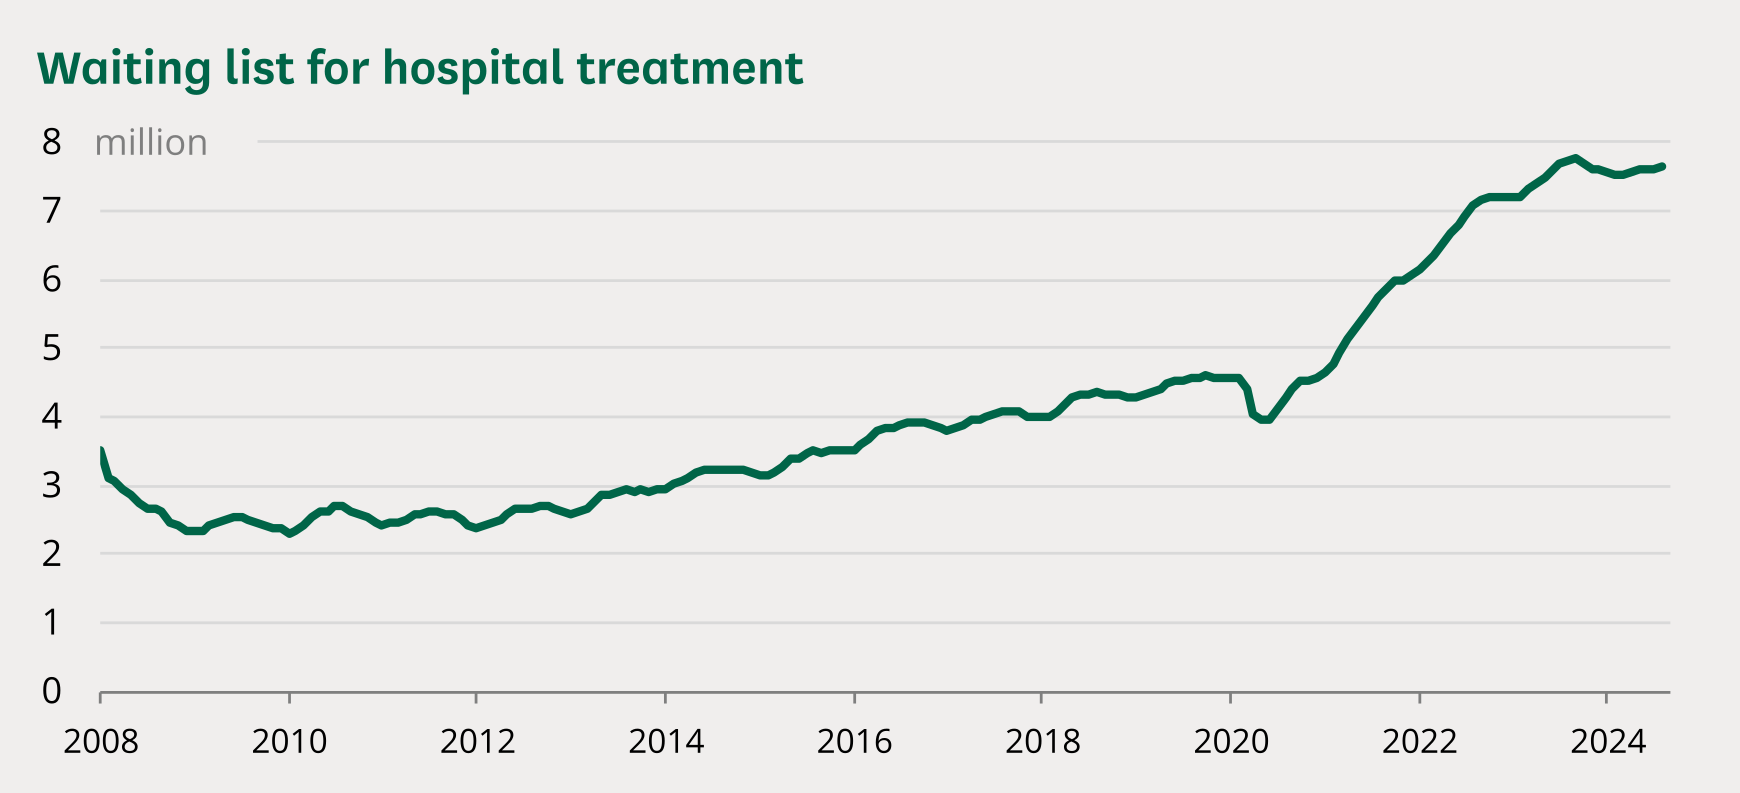
\includegraphics[width=1\linewidth]{img/Figuur-0.png}
    \caption{Wachtlijst voor ziekenhuisbehandeling (2011 - 2024)}
    \label{fig:Figuur0}
    \textit{Source: \autocite{Stiebahl2024}}
\end{figure}

%---------- Stand van zaken ---------------------------------------------------

\section{Literatuurstudie}%
\label{sec:literatuurstudie}

%Hier beschrijf je de \emph{state-of-the-art} rondom je gekozen onderzoeksdomein, d.w.z.\ een inleidende, doorlopende tekst over het onderzoeksdomein van je bachelorproef. Je steunt daarbij heel sterk op de professionele \emph{vakliteratuur}, en niet zozeer op populariserende teksten voor een breed publiek. Wat is de huidige stand van zaken in dit domein, en wat zijn nog eventuele open vragen (die misschien de aanleiding waren tot je onderzoeksvraag!)?

%Je mag de titel van deze sectie ook aanpassen (literatuurstudie, stand van zaken, enz.). Zijn er al gelijkaardige onderzoeken gevoerd? Wat concluderen ze? Wat is het verschil met jouw onderzoek?

% Verwijs bij elke introductie van een term of bewering over het domein naar de vakliteratuur, bijvoorbeeld~\autocite{Hykes2013}! Denk zeker goed na welke werken je refereert en waarom.

%Draag zorg voor correcte literatuurverwijzingen! Een bronvermelding hoort thuis \emph{binnen} de zin waar je je op die bron baseert, dus niet er buiten! Maak meteen een verwijzing als je gebruik maakt van een bron. Doe dit dus \emph{niet} aan het einde van een lange paragraaf. Baseer nooit teveel aansluitende tekst op eenzelfde bron.

%Als je informatie over bronnen verzamelt in JabRef, zorg er dan voor dat alle nodige info aanwezig is om de bron terug te vinden (zoals uitvoerig besproken in de lessen Research Methods).

% Voor literatuurverwijzingen zijn er twee belangrijke commando's:
% \autocite{KEY} => (Auteur, jaartal) Gebruik dit als de naam van de auteur
%   geen onderdeel is van de zin.
% \textcite{KEY} => Auteur (jaartal)  Gebruik dit als de auteursnaam wel een
%   functie heeft in de zin (bv. ``Uit onderzoek door Doll & Hill (1954) bleek
%   ...'')

%Je mag deze sectie nog verder onderverdelen in subsecties als dit de structuur van de tekst kan verduidelijken.


In de laatste decennia zijn de wachttijden voor de A\&E afdelingen binnen de NHS substantieel toegenomen zoals aangetoond in fig. \ref{fig:Figuur1}. Een recent onderzoek uitgevoerd door \autocite{Baker2024} toont een sterke toename in het percentage van patiënten die meer dan vier uur spenderen in de A\&E afdeling, en dit tussen 2015 en 2020. Sindsdien is er een nieuw record bereikt met 50,4\% van patiënten die meer dan vier uur doorbrengen in de A\&E afdeling. Dit vormt een duidelijke overtreding van de 4-uur norm van de NHS. Deze richtlijn houdt in dat tenminste 95\% van de patiënten binnen vier uur moeten worden opgenomen, overgebracht en ontslagen. \autocite{NationalStatisticsONS2024}.


\begin{figure}[h]
    \centering
    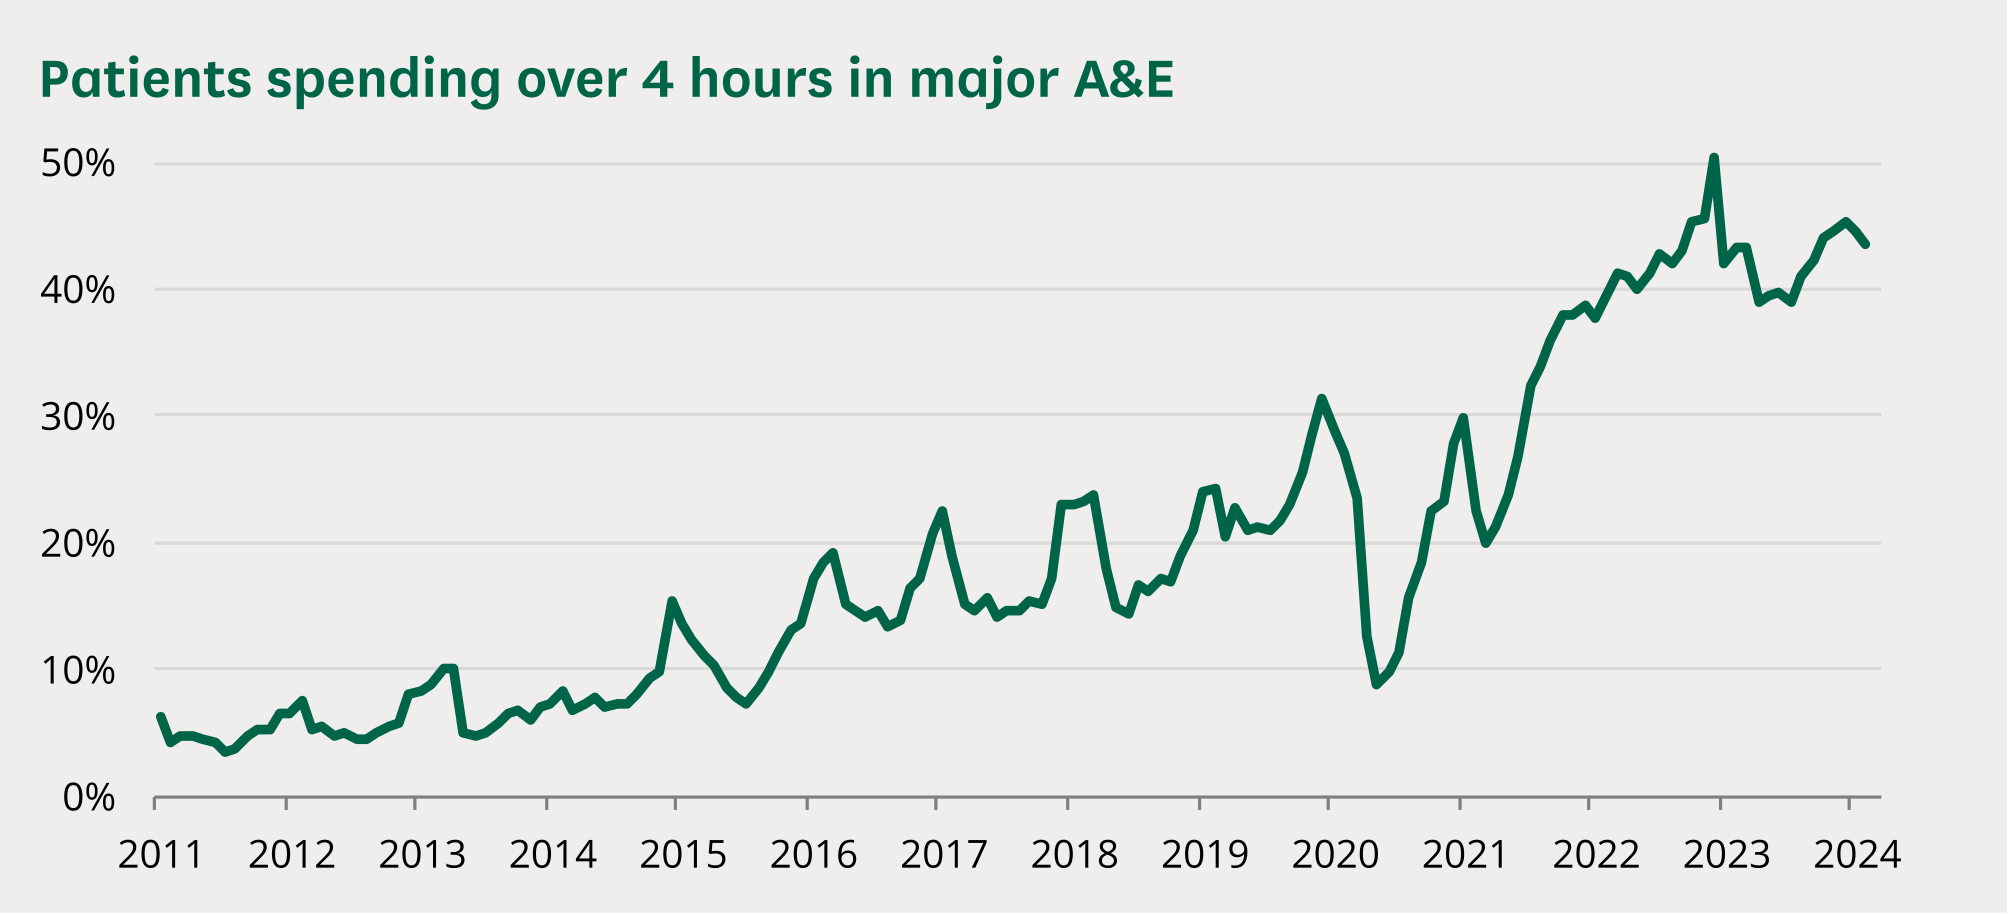
\includegraphics[width=1\linewidth]{img/Figuur-1.png}
    \caption{Percentage van patiënten die meer dan 4 uur spenderen in de A\&E departement}
    \label{fig:Figuur1}
    \textit{Source: \autocite{Baker2024}}
\end{figure}


Niet voldoen aan deze richtlijn heeft serieuze gevolgen voor de zorgkwaliteit en patiëntentevredenheid zoals aangetoond door \autocite{Vainieri2020}. Volgens de bevindingen van \autocite{Paling2020} zijn de implicaties echter veel ernstiger. De studie vermeldt dat lange wachttijden in de A\&E afdeling een verband toont met complicaties en mortaliteit onder patiënten. De oorzaak volgens \autocite{Paling2020}, is te wijten aan een hoge beddenbezettingsgraad. Verder toont het onderzoek een correlatie tussen de hoge beddenbezetting en de lange wachttijden in de A\&E afdeling zoals aangetoond door fig. \ref{fig:Figuur2}.


\begin{figure}[h]
    \centering
    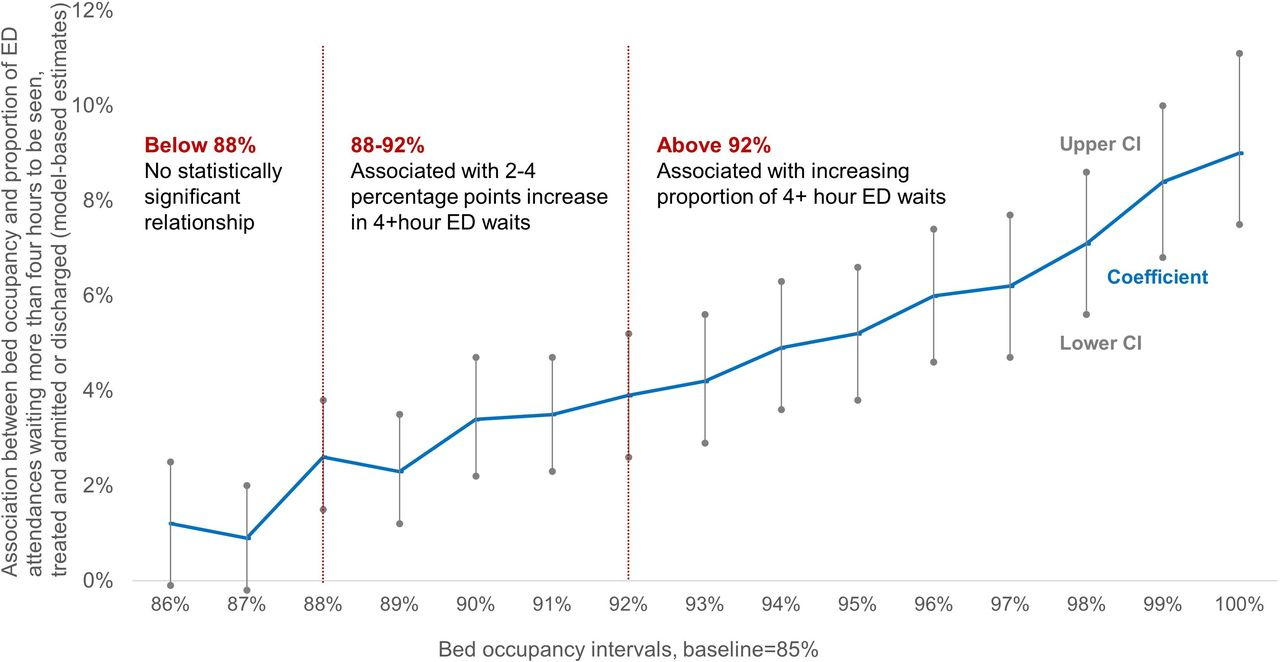
\includegraphics[width=0.5\textwidth]{img/Figuur-2}
    \caption{Plot dat een niet-lineaire relatie toont tussen bedbezettingen intervallen en proportie van patienten die meer dan 4 uur spenderen in de A\&E departement}
    \label{fig:Figuur2}
    \textit{Source: \autocite{Paling2020}}
\end{figure}

Patiënten zijn niet de enigen die worden beïnvloed door de langdurige wachttijden; onderzoekers hebben onlangs de werkomstandigheden van NHS werknemers onderzocht. De studie toont dat 40\% van alle ziekten bij het personeel te wijten is aan stress. Verder wijst het onderzoek uit dat de “overheersende stressfactor” wordt veroorzaakt door de hoge werkdruk \autocite{Ravalier2020}. \autocite{Vainieri2020} onderlijnt overbevolking als oorzaak van de hoge werkbelasting, en dit in A\&E departementen in diverse westerse landen. Om beter te begrijpen hoe IoT dit probleem kan oplossen, is het noodzakelijk om dieper in te gaan op wat IoT precies inhoudt. Over het algemeen verwijst Internet of things (IoT) naar een model dat verschillende technologieën omvat. Anders gezegd, is het een netwerk van elektronische apparaten die met elkaar of met de cloud communiceren via het internet. De afgelopen twee decennia hebben een grote invloed gehad op de snelle vooruitgang van IoT \autocite{Almutairi2024}, hierdoor is het aantal aangesloten IoT devices sterk gestegen, met 7.74 miljard in 2019, 10.7 miljard in 2021 \autocite{Dawod2022} en 25.44 miljard tegen 2030 \autocite{Dawod2022}. Sensoren, camera's en gelijkaardige apparaten worden al “geïntegreerd” in “woningen” en “voertuigen” \autocite{Dawod2022} en geïmplementeerd over verschillende sectoren zoals de “gezondheidszorg, landbouw, productie” en slimme steden \autocite{Almutairi2024}.

De implementatie van miljarden \autocite{Dawod2022} IoT devices over verschillende sectoren geeft een duidelijke representatie van de veranderingen die IoT zal brengen in de manier waarop men leeft, werkt en omgaat met de omgeving \autocite{Almutairi2024}. De vraag is nu of IoT gebruikt kan worden in de gezondheidszorg om wachttijden in de Accident \& Emergency afdelingen te verkorten. Volgens een recente studie uitgevoerd door \autocite{Singh2023} is het perfect mogelijk om IoT te implementeren in de gezondheidszorg. Echter concludeert het onderzoek dat IoT een gunstige invloed heeft en dit ondanks de beperkingen in “energie, processing en opslag”. Verder benadrukt de studie dat IoT een “veelbelovende technologie” is bij het besparen van tijd en moeite voor het medische personeel. 

%----------------------------------------------------------------------------------------------------------------------

IoT kan op verschillende manieren worden ingezet in de gezondheidszorg \autocite{Huang2021}. Ten eerste kan IoT ingezet worden voor het beheren van medische uitrusting, medicatie en data. Vervolgens door gebruik te maken van IoT ondersteunende slimme apparaten en systemen kan de patiëntenstroom worden beheerd \autocite{Almotaira2023} en patiënten pieken voorspeld \autocite{King2022}. De werking hiervan, zoals aangetoond in fig. \ref{fig:Figuur4} is als volgt, iedere patiënt beschikt over zijn eigen IoT device, zoals een sensor of een netwerk device. De device is vervolgens verbonden met een intelligente gateway, ook wel IoT gateway genoemd. Deze gateway zorgt voor communicatie tussen devices, en tussen device en cloud \autocite{Upadrista2021}. De gateway is verbonden met een datacollectie- en processing center via het internet, deze is verantwoordelijk voor het verwerken van ruwe data door de “correctheid” en “kwaliteit” te verbeteren om deze geschikt voor analyse te maken \autocite{Sirisha2023}. Eenmaal de ruwe data verwerkt, worden deze geanalyseerd en maakt het systeem beslissingen, die vervolgens door artsen en dokters gebruikt kunnen worden \autocite{Singh2023}. Kortom, verzamelen IoT apparaten realtime patiëntgegevens die geanalyseerd zijn om inzichten te verkrijgen en trends te voorspellen \autocite{Alrehaili2023, Sidhu2023}. 

\begin{figure}[h]
    \centering
    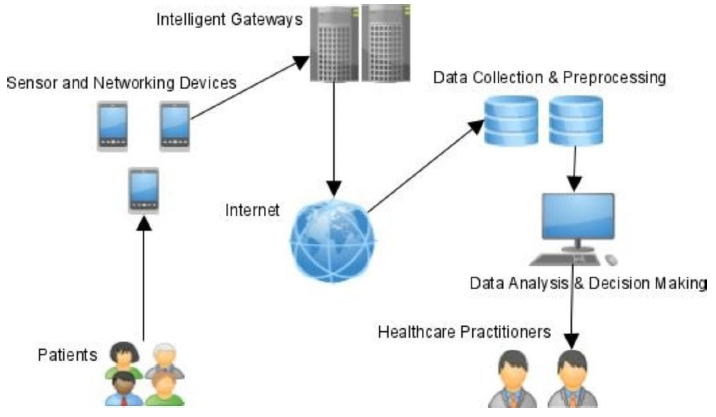
\includegraphics[width=0.5\textwidth]{img/Figuur-4}
    \caption{Internet of things (IoT) systeem in de gezondheidszorg}
    \label{fig:Figuur4}
    \textit{Source: \autocite{Singh2023}}
\end{figure}

%---------- Methodologie ------------------------------------------------------
\section{Methodologie}%
\label{sec:methodologie}

% Hier beschrijf je hoe je van plan bent het onderzoek te voeren. Welke onderzoekstechniek ga je toepassen om elk van je onderzoeksvragen te beantwoorden? Gebruik je hiervoor literatuurstudie, interviews met belanghebbenden (bv.~voor requirements-analyse), experimenten, simulaties, vergelijkende studie, risico-analyse, PoC, \ldots?

% Valt je onderwerp onder één van de typische soorten bachelorproeven die besproken zijn in de lessen Research Methods (bv.\ vergelijkende studie of risico-analyse)? Zorg er dan ook voor dat we duidelijk de verschillende stappen terug vinden die we verwachten in dit soort onderzoek!

% Vermijd onderzoekstechnieken die geen objectieve, meetbare resultaten kunnen opleveren. Enquêtes, bijvoorbeeld, zijn voor een bachelorproef informatica meestal \textbf{niet geschikt}. De antwoorden zijn eerder meningen dan feiten en in de praktijk blijkt het ook bijzonder moeilijk om voldoende respondenten te vinden. Studenten die een enquête willen voeren, hebben meestal ook geen goede definitie van de populatie, waardoor ook niet kan aangetoond worden dat eventuele resultaten representatief zijn.

%Uit dit onderdeel moet duidelijk naar voor komen dat je bachelorproef ook technisch voldoen\-de diepgang zal bevatten. Het zou niet kloppen als een bachelorproef informatica ook door bv.\ een student marketing zou kunnen uitgevoerd worden.

% Je beschrijft ook al welke tools (hardware, software, diensten, \ldots) je denkt hiervoor te gebruiken of te ontwikkelen.

%Probeer ook een tijdschatting te maken. Hoe lang zal je met elke fase van je onderzoek bezig zijn en wat zijn de concrete \emph{deliverables} in elke fase?

Dit onderzoek heeft als doel om aan te tonen of IoT in staat is om de wachttijden op de A\&E afdelingen van de NHS te verkorten.

\subsubsection*{Oorzakenanalyse}
Het onderzoek begint met het uitvoeren van een uitgebreide oorzakenanalyse. Dit is een fundamentele stap bij het identificeren van de oorzaak van de langdurige wachttijden binnen de A\&E afdelingen van ziekenhuizen. De analyse begint met het definiëren van het probleem. Om die reden wordt de “5 Whys”-methode toegepast samen met een brain\-storming-sessie. De “5 Whys”-methode wordt gebruikt om de kern van het probleem te achterhalen door telkens de vraag waar\-om te stellen, \ref{fig:Figuur5} en de oorzaak proberen te identificeren via de brain\-storming-sessie. Zodra diverse oorzaken geïdentificeerd zijn, begint er een analyse door middel van het Fishbone-model. De reden achter het gebruik van dit model is het voorkomen dat mogelijke onderliggende oorzaken over het hoofd worden gezien. Verder biedt het model simpliciteit bij het trekken van conclusies dankzij een visuele representatie tussen de categorisch weergegeven oorzaken en het probleem. Vervolgens is elke oorzaak zorgvuldig bestudeerd, degene die de grootste impact heeft op langdurige wachttijden is geselecteerd als de hoofdoorzaak. Een overweging is vervolgens gemaakt, om te achterhalen of IoT in het algemeen een oplossing kan zijn voor deze oorzaak. Verder in het onderzoek wordt er dieper bekeken naar welke IoT devices gebruikt kunnen worden in de gezondheidszorg, zodra de devices geselecteerd zijn, wordt er op een meer diepgaande wijze bekeken hoe de apparaten een oplossing kunnen zijn voor de hoofdoorzaak.

\begin{figure}[h]
    \centering
    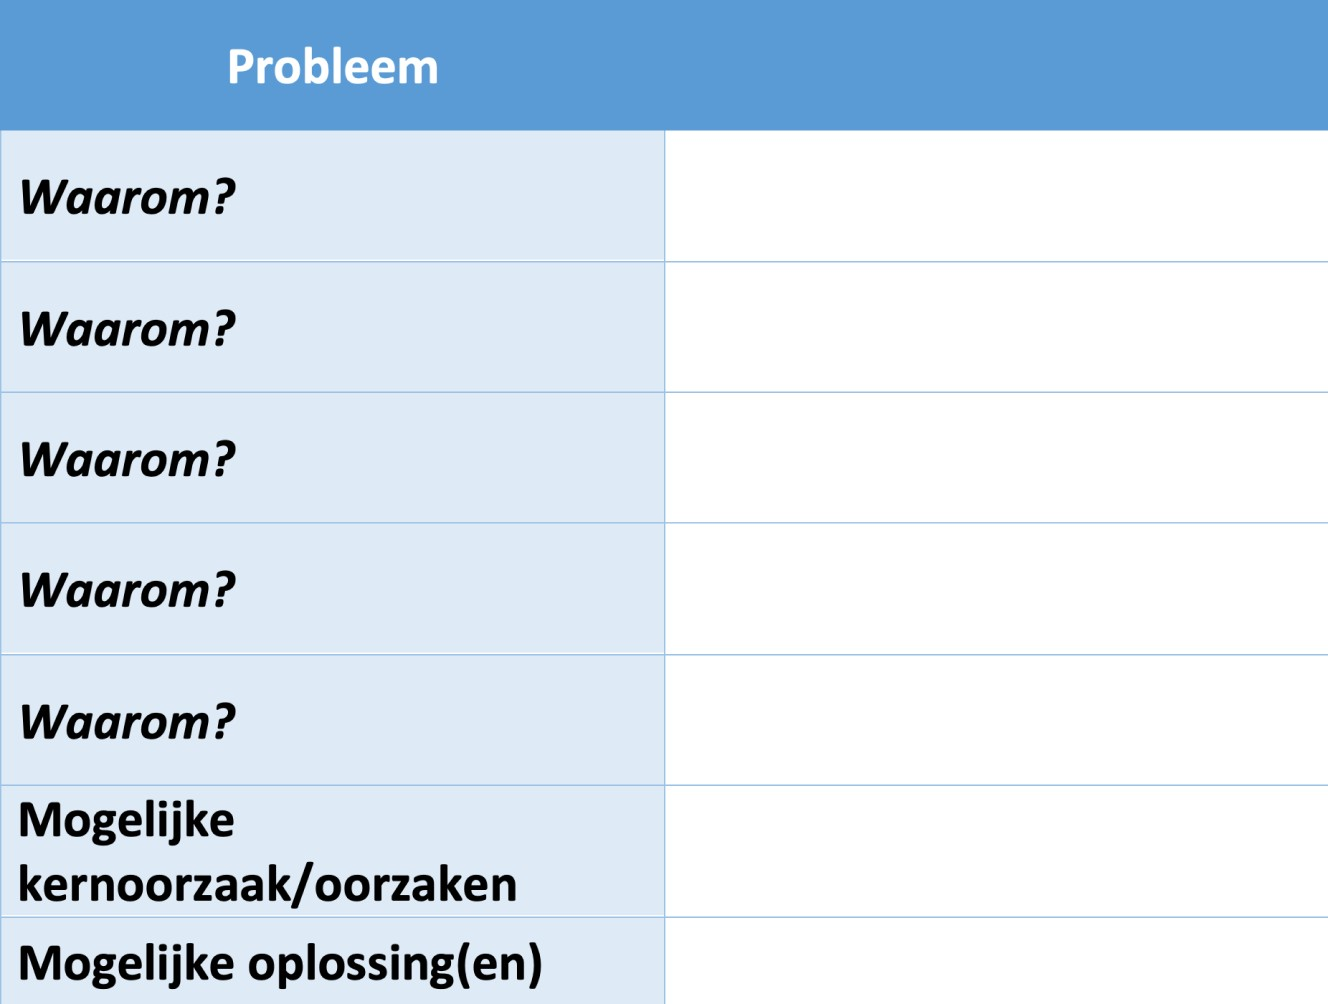
\includegraphics[width=0.5\textwidth]{img/Figuur-5}
    \caption{5 Whys”-methode}
    \label{fig:Figuur5}
    \textit{Source: \autocite{Scharwaechter2023}}
\end{figure}

\begin{figure}[h]
    \centering
    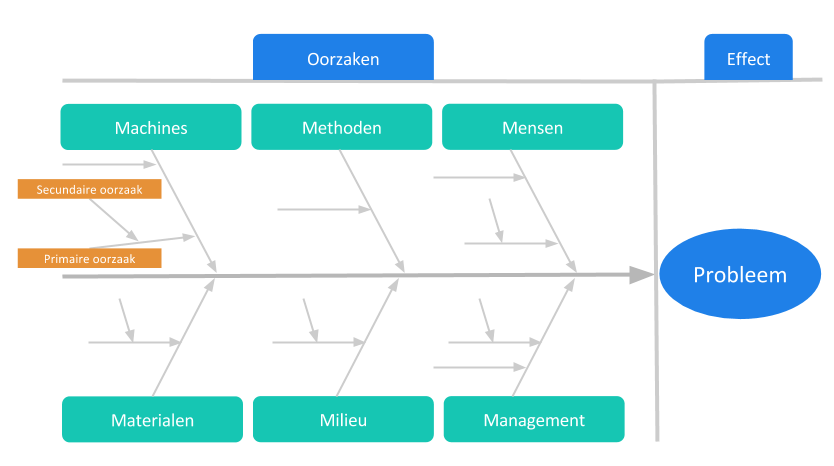
\includegraphics[width=0.5\textwidth]{img/Figuur-6}
    \caption{De fishbone diagram (ook de Ishikawa diagram genoemd)}
    \label{fig:Figuur6}
    \textit{Source: \autocite{Swaen2023}}
\end{figure}

\subsubsection*{Case study}
Deze case study wordt uitgevoerd als toelichting voor het implementeren van IoT technologieën. De primaire doelstelling van deze case study is het identificeren van praktische voorbeelden van IoT gebruik om lange wachttijden in A\&E afdelingen te verminderen. Daarnaast richt de case study zich op het identificeren van verschillende IoT apparaten die ingezet kunnen worden om wachttijden verder te verkorten. De case study begint met het identificeren van specifieke casussen. Na het vaststellen van een casus worden er kwalitatieve en kwantitatieve gegevens verzameld over de gekozen casus, dit houdt in dat verschillende bronnen worden geraadpleegd bij het verzamelen van informatie zoals wetenschappelijke literatuur, rapporten van gezondheidsorganisaties, archieven en documenten. Na het vaststellen van diverse casussen worden deze geanalyseerd en de gebruikte IoT-devices en IoT categorieën opgelijst. Verder worden gegevens verzameld voor elk van de opgelijste devices, verschillende bronnen zoals onderzoeksrapporten, literatuurstudies, academische tijdschriften en technologische onderzoeken worden hiervoor geraadpleegd. 

\subsubsection*{Identificeren van IoT-devices}
Het identificeren van IoT apparaten is van het uiterste belang, daarom is er aanzienlijk veel tijd besteed aan het opstellen van de casestudie om een assortiment van IoT apparaten te bepalen. Dit houdt in dat elk device grondig bestudeerd zal worden om een beter begrip te krijgen in de werking hiervan in de gezondheidszorg. Om het meest gepaste IoT device te selecteren worden verschillende IoT categorieën bekeken, deze categorieën vertegenwoordigen IoT apparaten die de werking van de A\&E afdelingen kunnen verbeteren en efficiënter maken, deze categorieën zijn: Locatie- en traceerapparaten, Communicatieapparaten, Integratie van het gegevensbeheer en Integratie en coördinatie van IoT devices. De categorieën worden geselecteerd op basis van de nodige IoT devices in de proof-of-concept. Het Real-time Smart Queue Management System maakt gebruik van bewegings- en aanwezigheidssensoren, die worden ingezet om de locatie van patiënten in de wachtrij in real-time te volgen.

\subsubsection*{Vergelijkende analyse}
In deze sectie worden de geïdentificeerde IoT devices met elkaar vergeleken om de meest geschikte keuze voor de Proof-of-Concept te bepalen. De vergelijking is gebaseerd op de volgende criteria:

\begin{itemize}
    \item \textbf{Voor- en nadelen:} Een gedetailleerde lijst van de voordelen en nadelen van elk apparaat wordt opgesteld. Dit bevat de prestatie, veiligheid, en specifieke toepassingen.
    
    \item \textbf{Kosten:} De kostenanalyse omvat enkel de aanschafkosten.
    
    \item \textbf{Betrouwbaarheid:} Hier wordt gekeken naar de stabiliteit van het apparaat, de frequentie van uitval, de kwaliteit van de hardware, evenals de beschikbaarheid van technische ondersteuning.
    
    \item \textbf{Gebruiksvriendelijkheid:} Dit criterium omvat de eenvoud van installatie, configuratie, bediening.

    \item \textbf{Integratie capaciteit:} De mogelijkheid om het IoT apparaat te integreren met andere systemen of apparaten (Raspberry Pi, Arduino) wordt onderzocht. 
\end{itemize}

\paragraph*{Methodologie van vergelijking}
Voor een objectieve vergelijking wordt gebruik gemaakt van een matrix of tabel waarin elk apparaat op elk criterium wordt beoordeeld.

\paragraph*{Resultaten en Conclusie}
De resultaten van deze vergelijking leiden tot een aanbeveling voor de meest geschikte IoT devices voor de Proof-of-Concept. Deze aanbeveling wordt ondersteund door een uitgebreide uitleg van waarom bepaalde devices de voorkeur krijgen boven andere, met speciale aandacht voor hoe ze bijdragen aan de doelstellingen van het project.

\subsubsection*{Selectie ziekenhuis}
Voordat de Proof-of-Concept wordt uitgevoerd, wordt er een ziekenhuis gezocht, bij voorkeur in Vlaanderen. Een ziekenhuis wordt geselecteerd op basis van de bereidheid om samen te werken en de beschikbaarheid van een geschikte spoedafdeling voor het testen van het systeem. De spoedafdeling moet beschikken over een wachtzaal met voldoende capaciteit voor patiënten en benodigde sensoren. Om de samenwerking te vergemakkelijken, kan de Proof-of-Concept worden aangepast zodat deze volledig voldoet aan de geldende GDPR-richtlijnen van het ziekenhuis.

\subsubsection*{Proof-of-Concept: Real-Time Smart Queue Management systeem met IoT}
Real-time Smart Queue Management systeem wordt ingezet om te onderzoeken of IoT een positief effect heeft op het verkorten van lange wachttijden binnen de NHS. De proof-of-concept (PoC) van het smart queue management systeem maakt gebruik van een Raspberry Pi die als hoofdcontroller fungeert, verbonden met een Arduino. De Arduino bestuurt verschillende sensoren in de wachtruimte, die bewegingen en de aanwezigheid van patiënten detecteren zonder persoonlijke gegevens te verzamelen. Het systeem maakt gebruik van beweging- en aanwezigheidssensoren die anoniem de aanwezigheid van patiënten in de wachtruimte detecteert. De sensoren worden strategisch geplaatst bij de ingangen en tussen verschillende secties van de wachtruimte. Wanneer een patiënt de ruimte betreedt, registreert het systeem een tijdstempel van deze beweging. Dit gebeurt ook wanneer een patiënt zich verplaatst of de ruimte verlaat. Om dubbele tellingen te voorkomen wordt er een Lichtsluis of infraroodsensoren gebruikt bij doorgangen, waarmee de richting van de beweging (in- of uitgang) nauwkeurig wordt gedetecteerd. Voor de monitoring van zittende patiënten worden druksensoren onder de stoelen geplaatst. Deze detecteren of een stoel bezet is en helpen om het totaal aantal aanwezige patiënten nauwkeurig bij te houden zonder onnodige activering van andere bewegingssensoren. Voor het detecteren van patiënten die staan, wordt gebruikgemaakt van een thermische camera. Dit biedt een betrouwbaar en privacyvriendelijk middel om warmtepatronen te detecteren en onderscheid te maken tussen individuele personen en groepen zonder het gebruik van persoonlijke gegevens. De Arduino(s) verzendt de gegevens naar de Raspberry Pi via een seriële verbinding of draadloze protocol voor verwerking. De Raspberry Pi verwerkt de gegevens met behulp van een Python-script en berekent de volgorde en wachttijden van patiënten in de wachtruimte op basis van de tijdstempels. De gegevens worden vervolgens naar een cloudgebaseerd platform zoals een MQTT-server of een tijdreeksdatabase (bijvoorbeeld InfluxDB) verzendt. Deze data kan real-time worden geanalyseerd om de wachttijden te berekenen en om te bepalen welke patiënt als volgende aan de beurt is. Om de kans op false-positives en onnauwkeurige data te minimaliseren, worden technieken zoals filtering (om ruis te verminderen) en debouncing (om fluctuaties in digitale signalen te stabiliseren) toegepast op de sensorgegevens.

Een dashboard visualiseert en bewerkt de wachtrijstatus in real-time, inclusief:

\begin{itemize}
    \item Het totale aantal patiënten in de wachtruimte.
    \item De geschatte wachttijd per patiënt.
\end{itemize}

Het dashboard geeft het ziekenhuispersoneel gedetailleerde informatie over het aantal patiënten in de wachtruimte, de geschatte wachttijd per patiënt en de volgorde van behandeling. Dit zorgt ervoor dat het personeel steeds prioriteit kan geven aan de patiënt die het langst wacht. Om patiënten te informeren over de status van de wachtrij, wordt er in de wachtruimte een scherm geplaatst dat in real-time de positie van de patiënten in de wachtrij en hun resterende wachttijd toont via een webinterface die verbonden is met het cloudplatform. De PoC zal uitgevoerd worden op een spoedafdeling in Vlaanderen, waarbij gebruik wordt gemaakt van sensoren en een cloudgebaseerd platform.

\subsubsection*{Evaluatie}
Na de PoC wordt er een evaluatie uitgevoerd om de effectiviteit van de PoC vast te stellen. De evaluatie zal beginnen met het vaststellen van een baseline van de huidige gemiddelde wachttijden. Dit wordt gedaan door het raadplegen van het personeel of beschikbare documentatie, indien aanwezig. Als deze gegevens niet beschikbaar zijn, zal er een nulmeting uitgevoerd worden op een dag met een gemiddeld of hoog patiëntenaantal. Tijdens deze nulmeting worden de tijdstippen van binnenkomst en oproep van elke patiënt handmatig of automatisch geregistreerd om de totale wachttijd nauwkeurig te bepalen. Na implementatie van de PoC worden dezelfde meetmethoden toegepast over een vergelijkbare periode om de impact van het systeem te meten. De resultaten van beide metingen worden vergeleken om vast te stellen of de PoC een vermindering van de gemiddelde wachttijden heeft opgeleverd. Hierbij wordt rekening gehouden met eventuele variabelen die de wachttijd kunnen beïnvloeden, zoals piekmomenten en personeelsbezetting.

\subsubsection*{Resultaten}

De resultaten worden beschouwd als een succes, indien de proof-of-concept duidelijk aantoont dat IoT gebruikt kan worden bij het verminderen van de wachttijden.

%\begin{figure}[h]
%    \centering
%    \subsubsection*{Milestone} % Place the subsection above the figure
%    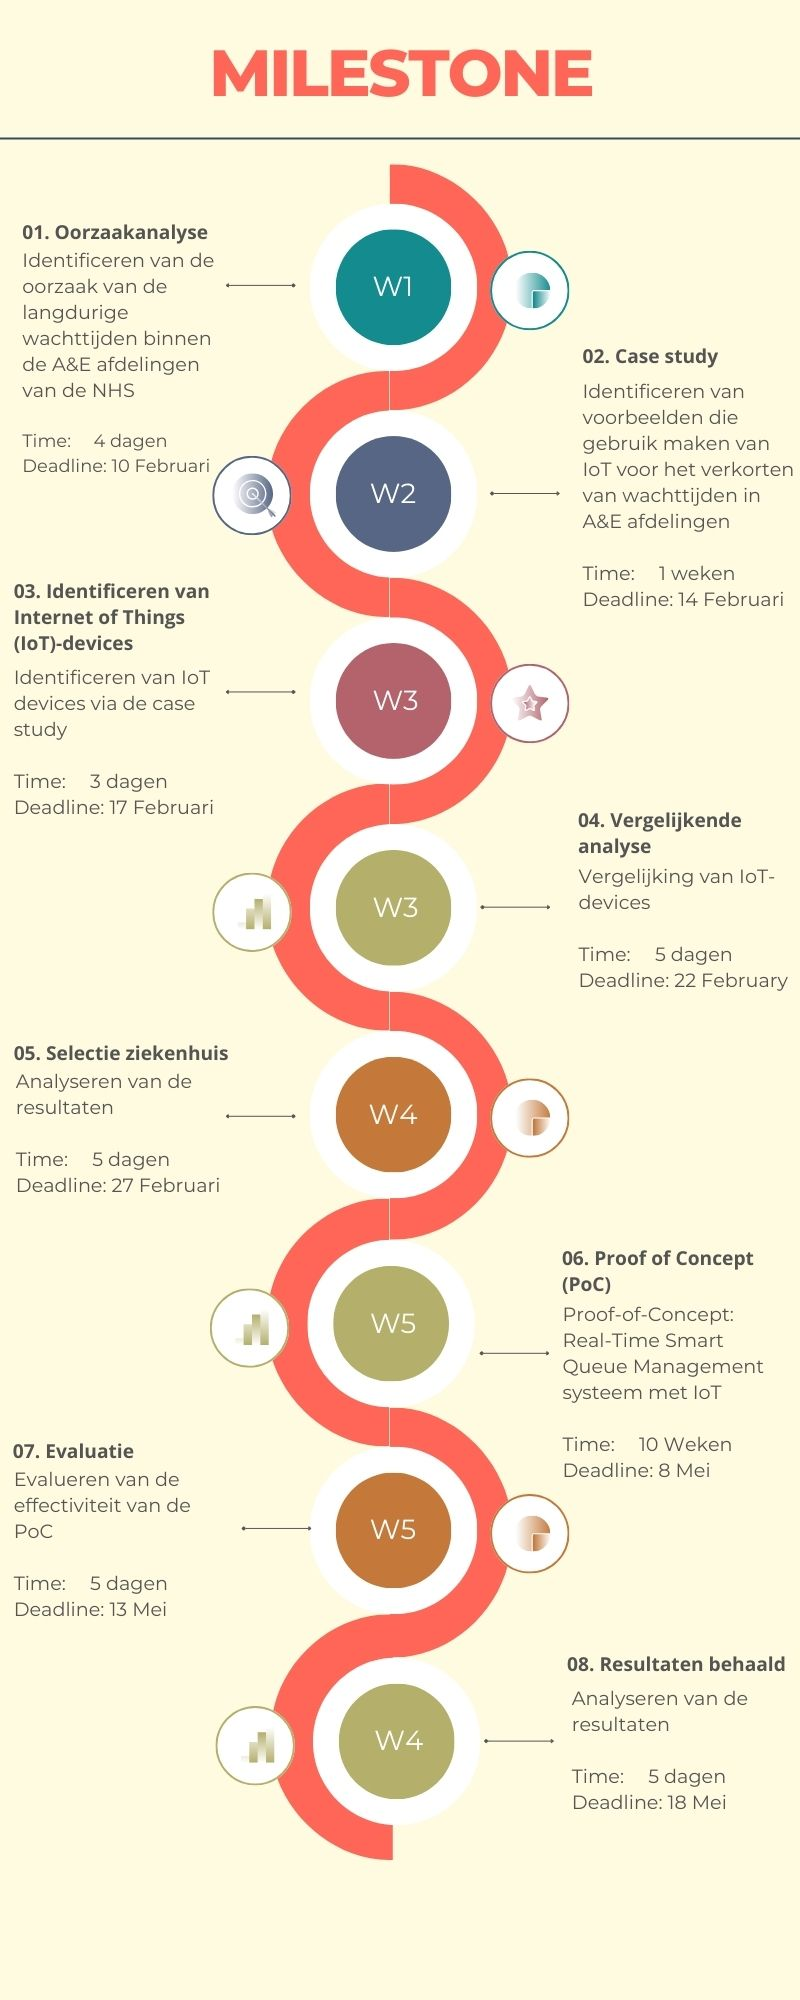
\includegraphics[width=0.92\linewidth]{img/milestone-4.png}
%    \label{fig:Figuur8}
%\end{figure}



%---------- Verwachte resultaten ----------------------------------------------
\section{Verwacht resultaat, conclusie}%
\label{sec:verwachte_resultaten}

% Hier beschrijf je welke resultaten je verwacht. Als je metingen en simulaties uitvoert, kan je hier al mock-ups maken van de grafieken samen met de verwachte conclusies. Benoem zeker al je assen en de onderdelen van de grafiek die je gaat gebruiken. Dit zorgt ervoor dat je concreet weet welk soort data je moet verzamelen en hoe je die moet meten.

% Wat heeft de doelgroep van je onderzoek aan het resultaat? Op welke manier zorgt jouw bachelorproef voor een meerwaarde?

% Hier beschrijf je wat je verwacht uit je onderzoek, met de motivatie waarom. Het is \textbf{niet} erg indien uit je onderzoek andere resultaten en conclusies vloeien dan dat je hier beschrijft: het is dan juist interessant om te onderzoeken waarom jouw hypothesen niet overeenkomen met de resultaten.

De verwachte resultaten voor dit onderzoek is dat de proof-of-concept duidelijk aantoont of IoT in staat is om de wachttijden te verkorten. Als de proof-of-concept kan bewijzen dat IoT de wachttijden verkort kan zijn dan wordt er geconcludeerd dat IoT in staat is om significante verbeteringen te brengen aan de wachttijden, in alle andere gevallen wordt het tegenovergestelde geconcludeerd. De resultaten die hieruit volgen kunnen een duidelijke meerwaarde bieden voor ziekenhuizen die IoT evalueren als oplossing tegen lange wachttijden.
